%\documentclass{scrartcl}[a4paper, 12pt]
\documentclass[
	english,
	ruledheaders=section,%Ebene bis zu der die Überschriften mit Linien abgetrennt werden, vgl. DEMO-TUDaPub
	class=report,% Basisdokumentenklasse. Wählt die Korrespondierende KOMA-Script Klasse
	thesis={type=Proposal},% Dokumententyp Thesis, für Dissertationen siehe die Demo-Datei DEMO-TUDaPhd
	accentcolor=9c,% Auswahl der Akzentfarbe
	custommargins=true,% Ränder werden mithilfe von typearea automatisch berechnet
	marginpar=false,% Kopfzeile und Fußzeile erstrecken sich nicht über die Randnotizspalte
	%BCOR=5mm,%Bindekorrektur, falls notwendig
	parskip=half-,%Absatzkennzeichnung durch Abstand vgl. KOMA-Script
	fontsize=11pt,%Basisschriftgröße laut Corporate Design ist mit 9pt häufig zu klein
	%logofile=example-image, %Falls die Logo Dateien nicht vorliegen
]{tudapub}

\usepackage{amsmath}
\usepackage{amssymb}
\usepackage{bbold}
\usepackage{slashed}

\usepackage{float}

\graphicspath{ {images/} }
\usepackage{graphicx} % Required for inserting images
%\usepackage{todonotes}
\newcommand{\todoin}{\todo[inline]}
\usepackage[disable]{todonotes}
\newcommand{\redtodo}{\textcolor{red}{TODO}}

\newcommand{\sqbr}[1]{\left[#1\right]}
\newcommand{\rbr}[1]{\left(#1\right)}
\newcommand{\cbr}[1]{\left\{#1\right\}}

%rectangle
\newcommand{\rectangle}{{\mathbin{\scalebox{2}[1]{$\square$}}}}

\usepackage{mathtools}
\DeclarePairedDelimiter\bra{\langle}{\rvert}
\DeclarePairedDelimiter\ket{\lvert}{\rangle}
\DeclarePairedDelimiterX\braket[2]{\langle}{\rangle}{#1\,\delimsize\vert\,\mathopen{}#2}

\DeclareMathOperator{\tr}{tr}

\newcommand{\lagr}{\mathcal L}

\begin{document}

\title{High-Precision Pressure Measurement in Full Lattice QCD for $N_f=2+1$}
\author{Abdelhamid Ettahri}
\reviewer{Guy D. Moore}
%\date{December 2025}
\submissiondate{February 24, 2026}

\department{Fachbereich Physik}
\institute{Institut für Kernphysik: Theoriezentrum}
\group{AG Moore}

\maketitle

\chapter*{Abstract}In this thesis, we prepare all the tools needed to do a high-precision measurement of the pressure in a Quark-Gluon plasma using Lattice Quantum Chromodynamics (QCD) for $N_f=2+1$ using the tree level symanzik improved gauge action and the HISQ fermion action. We first introduce the continuum quantum field theory and how Lagrangian naturally arises from the free Dirac Lagrangian by enforcing $SU(3)$ gauge invariance. Afterwards, we look at the implementation of QCD on the lattice. This section is followed by a short review of statistical mechanics and the introduction of the integral method which will be used to achieve the precision measurement of the pressure. Then, we will look at Monte Carlo integration which will be used to do lattice measurements. Finally, we will end the thesis with an outlook of the planned lattice measurements.    \tableofcontents


\listoftodos    \todo[inline]{Rewrite introduction} \todo[author=Al]{Add figure}    \todo[color=yellow!30]{Clarify wording} \newpage


\chapter{Motivation}                            Quantum Chromodynamics (QCD) is a non-abelian gauge theory that describes the interactions between gluons and quarks. One of its central characteristics is the running of gauge coupling. At high energy scales, at which we have high-momentum transfer, the gauge coupling becomes very small resulting in gluons and quarks being almost free. This gives rise to the name asymptotic freedom. On the other hand we have a strong coupling for low-energy phenomena, in which the gluons and quarks cannot appear on their own, but only confined in hadrons\cite{bellac}. \\
The phase diagram of QCD is complicated and not fully understood. A sketch can be seen in figure \ref{fig:phase}. In very hot settings, for example at hundreds of MeV (trillions of Kelvin), hadron matter becomes deconfined and changes into the Quark-Gluon plasma (QGP). This state of matter occurs under extreme conditions such as in the core of heavy neutron stars and in ultra-relativistic heavy-ion collisions, which can be experimentally recreated in particle accelerators such as the LHC in CERN and RHIC in BNL\cite{phasediagram}. While understanding these phenomena is important on its own, it can also help to understand the early universe. Roughly $10^{-5}$\,s after the Big Bang matter was also a QGP\cite{monnai}.\\
\begin{figure}[H]
    \centering
    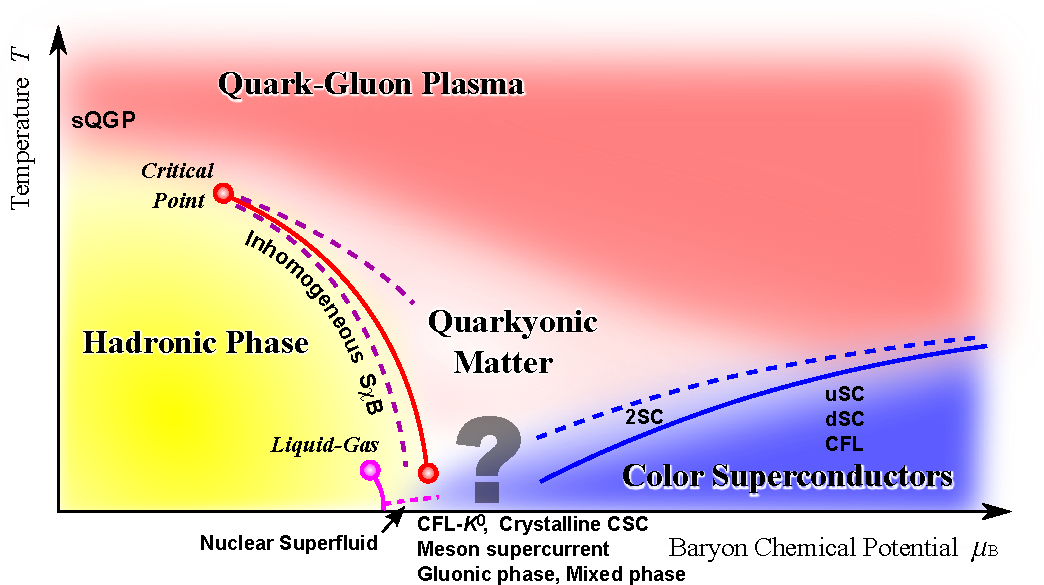
\includegraphics[width=0.7\linewidth]{images/phase.pdf}
    \caption{QCD Phase diagram \cite{phasediagram}}
    \label{fig:phase}
\end{figure}
Understanding these processes requires the equation of state, which is the reason for our calculation of the pressure in this thesis. To describe the theory in a more general setting, we would have to include the baryon chemical potential. However, this would make the calculation even more complicated, since its inclusion would invoke the sign problem which would make a direct lattice calculation impossible. Pavan et al. \cite{pavan} was able to compute the pressure for non-vanishing chemical potential. The uncertainties of their results are dominated by uncertainties of the literature values for the pressure for vanishing chemical potential. We hope to reduce these errors by providing a high precision measurement of the pressure for vanishing chemical potential.\\
A high-precision pressure measurement would also be useful and needed for the renormalization of the Energy-Momentum-Stress Tensor (EMT). The EMT can then be used to describe the hydrodynamics of the QGP. 


\newpage

\chapter{Quantum Chromodynamics}                

%\section{Introduction to QCD}
%In the Standard Model of Particle Physics there are four fundamental interactions, namely electromagnetism, the strong and weak interaction and finally gravitation. Ignoring gravitation, the other three forces can each be explained as a Quantum Field Theory (QFT)\cite{thomson}.\\ 
%While it is clear that the description of the interactions necessitates a quantum mechanical treatment, the need of the field viewpoint might be less obvious. One of the reasons for this, as mentioned in \cite{peskin}, is the fact that the processes of our interest are happening at relativistic energies, where we see the creation and annihilation of particles-antiparticle pairs, which cannot be easily explained when thinking of single particles.\\
%\todo[inline]{add: instead of starting with field operators we start with classical action and then put in path integral} 
\todo[inline]{Introduce the Standard Model including the fundamental particles and interactions}
\todo[inline]{State that QFT is necessary for a description of QCD since its a relativistic quantum theory and so on}

The Standard Model of Particle Physics states that all matter is made up of quarks and leptons (and the corresponding antiparticles) and that all interactions in nature are a result of the exchange of the force carriers. All matter constituents carry the weak charge and thus are influenced by the weak interaction, which is carried by the W and Z bosons. With the exception of the neutrinos, they all have a nonzero electric charge and thus feel the electro-magnetic force carried by the photon. However, only the quarks carry the color charge and thus are under the influence of the strong interaction, which is carried by the gluons.
While all forces have to be considered for a full description of a theory, on the scales that we are interested in, the strong force is dominant and thus will be the only force which we will discuss here.\\
It is not surprising that at these sizes a quantum mechanical description is necessary. But this is actually not enough, since a relativistic analysis is also required. But even choosing a relativistic equation of motion instead of the Schrödinger equation will result in the problem, that some effects, like particle-antiparticle creation and annihilation, cannot be directly described, although they are very important for relativistic theories.\\
The way out is to describe the fundamental forces via Quantum Field Theories. In the case of the strong interaction the theory is called \textit{Quantum Chromodynamics}.\cite{thomson}\\
In this thesis we will use natural units, meaning we set
\begin{equation}
    c=\hbar=1=k_B,
\end{equation}
where $k_B$ stands for the Boltzmann constant. Furthermore, Einsteins summation rule is always implied if not stated otherwise and the (-,+,+,+) metric is used for the Minkwoski space.



\section{The Dirac Equation}
\todoin{Start with the free Dirac Lagrangian since we are dealing with fermions, introducing 4-Spinor, gamma matrices and so on}


In this section we will not include the strong interaction but look instead at the free Dirac Equation which will describe free spin-1/2 fermions, which will be derived following the approach of \cite{thomson}. \\
As mentioned above, the Schrödinger equation fails to be relativistic invariant. Recalling that the free Schrödinger equation can be motivated by starting with the non-relativistic energy-momentum relation
\begin{equation}
    E=\frac{p^2}{2m}
\end{equation}
and then promoting energy and momentum to operators (in position space representation), e.g. 
\begin{equation}
    E \rightarrow i\partial_t,\qquad p_k \rightarrow -i\partial_k,
\end{equation}
it is not surprising that this equation cannot be used for a relativistic description. Trying to derive a relativistic theory with the same philosophy in mind, e.g. by starting with
\begin{equation}
    E^2=p^2+m^2,\label{eq:relEMRel}
\end{equation}
will result in the Klein-Gordon equation. While this equation is Lorentz invariant, it raises some other problems which make this theory not suitable to describe fermions.\\
As an alternative Paul Dirac proposed an equation that is first order in space and time
\begin{equation}
    \hat E\psi = \left(\vec \alpha \cdot \hat{\vec p}+\beta m\right)\psi.
\end{equation}
By enforcing that solutions $\psi$ of the equation should also describe the relativistic energy-momentum relation \eqref{eq:relEMRel} and that the operator $\hat E$ should be hermitian, it follows that $\alpha_i$ and $\beta$ are 4 mutually anticommuting traceless hermitian matrices of even dimensions greater than or equal to four. This implies that the wavefunction $\psi$ is a four dimensional Dirac spinor
\begin{equation}
    \psi =(\psi_1, \psi_2, \psi_3, \psi_4)^T.
\end{equation}
It can be shown, that such a wavefunction describes fermions that have spin 1/2.\\ 
Following custom we introduce the gamma matrices which are defined by
\begin{equation}
    \gamma^0\equiv \beta,\quad \gamma^1=\beta\alpha_x, \quad\gamma^2=\beta\alpha_y, \quad\gamma^3=\beta\alpha_z,
\end{equation}
which are defined unique only up to an unitary transformation. For specific calculations it might be useful to choose a specific representation, but usually it is enough to use their defining properties which can be summarized in the Clifford Algebra\footnote{The Clifford Algebra is also satisfied by non-hermitian gamma matrices.}
\begin{equation}
    \lbrace \gamma^\mu,\gamma^\nu\rbrace=2\eta^{\mu\nu}\mathbb{1}.
\end{equation}
While these objects are matrices, $\gamma^\mu$ transforms like a four vector, thus making
\begin{equation}
    p_\mu\gamma^\mu =:\slashed p
\end{equation}
a Lorentz scalar. The right-hand side of the equation above is the Feyman slash notation, which is used, when a four vector is contracted with the gamma matrices.
Using the 4-momentum operator $\hat P_\mu=(\hat E, -\hat {\vec p})=i(\partial_0, \partial_k)=i\partial_\mu$, we can finally bring the Dirac equation into the form
\begin{equation}
    (i\slashed \partial-m)\psi = 0 = (\slashed p -m)\psi,
\end{equation}
which is obviously Lorentz invariant.\\
The Dirac equation is just the equation of motion, but we actually need the corresponding Lagrangian. For this we first introduce the Adjoint Dirac Spinor 
\begin{equation}
    \bar\psi=\psi^\dagger \gamma^0,
\end{equation}
which is the second degree of freedom of our theory. The Lagrangian can now be reverse-engineered to be
\begin{equation}
    \lagr(\psi, \bar \psi) = \bar\psi(i\slashed \partial-m)\psi.\label{eq:freeDirac}
\end{equation}
This is the Lagrangian of the free Dirac field for a single spin 1/2-fermion, e.g. a quark. When we look at $N_f$ flavors of quarks, we introduce for each flavor a wave function, with a (potentially) different corresponding mass and write
\begin{equation}
    \lagr = \sum_{f=1}^{N_f}\bar\psi^{(f)}(i\slashed \partial-m)\psi^{(f)}.
\end{equation}










\section{SU(3) Gauge Symmetry}
The Lagrangian in equation \eqref{eq:freeDirac} is the Lagrangian for free fermions. Since we are interested in their interaction under the influence of the strong interaction, we need to couple the fermions to the interaction. In QED this follows naturally by assuming that the theory has a local $U(1)$ gauge symmetry. This means, that the Lagrangian is invariant when the fermion fields are transformed via
\begin{equation}
    \psi(x)\rightarrow \exp(i\alpha(x))\psi(x),
\end{equation}
for some complex scalar function $\alpha(x)$. This can be interpreted as a one dimensional complex rotation.\\
In QCD we assume a local $SU(3)$ gauge symmetry, under which the fermion fields are now rotated in a 3-dimensional vector space, the color space. This means that the fermion fields are now elements of the 3-dimensional color space. All degrees of freedom are now
\begin{equation}
    \psi^{(f)}(x)_{\alpha c}.
\end{equation}
We first differentiate with the $(f)$ superscript between the 6 quark flavors: up, down, strange, charm, top and bottom. Then we have the 4-dimensional space-time coordinate $x$. $\alpha$ denotes the component of the 4-dimensional spinor space and runs from 1 to 4 and $c$ denotes the component of the 3-dimensional color space and runs from 1 to 3. Thus, a quark with a specific flavor has 12 degrees of freedom at each space-time coordinate.\\
Returning to the issue of the gauge invariance, it should not come as a surprise that the Dirac Lagrangian is not invariant under local $SU(3)$ gauge symmetries, since it is not even invariant under $U(1)$ gauge symmetry. The fields transform via
\begin{equation}
    \psi(x)\rightarrow\Omega(x)\psi(x),\qquad \bar\psi(x)\rightarrow\bar\psi(x)\Omega(x)^\dagger=\bar\psi(x)\Omega(x)^{-1},
\end{equation}
with independent gauge transformations $\Omega(x)\in SU(3)$ at each coordinate $x$. Since these matrices are in $SU(3)$ their determinant is 1 and they are unitary, which means that they satisfy $\Omega(x)^\dagger=\Omega(x)^{-1}$. This implies that the mass term of the Dirac equation satisfies the gauge symmetry
\begin{equation}
    m\bar\psi(x)\psi(x)\rightarrow m\bar\psi(x)\Omega(x)^{-1}\Omega(x)\psi(x)=m\bar\psi(x)\psi(x).
\end{equation}
However, the derivative term is not invariant
\begin{align}
    \bar\psi(x)\partial_\mu\psi(x)&\rightarrow\bar\psi(x)\Omega(x)^{-1}\Omega(x)\partial_\mu\psi(x)+\bar\psi(x)\Omega(x)^{-1}\left(\partial_\mu\Omega(x)\right)\psi(x) \\
    &~=\bar\psi(x)\partial_\mu\psi(x)+\bar\psi\Omega(x)^{-1}\left(\partial_\mu\Omega(x)\right)\psi(x).
\end{align}
The reason for this failure lies in the fact that the derivative compares the field at two different coordinates without taking into account that both fields are independently rotated in the color space. To solve this problem we introduce a matrix $U(x,y)\in SU(3)$ defined by the transformation rule
\begin{equation}
    U(x,y)\psi(y)\rightarrow\Omega(x) U(x,y)\psi(y)   
\end{equation}
which means that it transforms according to
\begin{equation}
    U(x,y)\rightarrow \Omega(x)U(x,y)\Omega(y)^\dagger.
\end{equation}
This means that we take the field at position $y$ and transform it so that it matches the gauge rotation at position $x$. In $U(1)$, e.g. in the QED case, we would say that this comparator compensates the phase difference between coordinates $x$ and $y$. \\
$SU(3)$ is a Lie Group and thus its infinitesimal group elements can be written as
\begin{equation}
    U(x+\epsilon n,x)=\mathbb{1}-ig\epsilon n^\mu A_\mu^a t^a+\mathcal{O}(\epsilon^2),\label{eq:comparator1storder}
\end{equation}
where $t^a$ are the 8 generators of $SU(3)$, $g$ is the gauge coupling and $A_\mu^a$ are defined to be the gluon fields.\\
We can now define the covariant derivative that will substitute the usual derivative to recover gauge invariance. The  differential quotient will be changed to
\begin{equation}
    n^\mu D_\mu (x)= \underset{\epsilon\to0}{\lim} \frac{\psi(x+\epsilon n)-U(x+\epsilon n,x)\psi(x)}{\epsilon}.
\end{equation}
By the definition of the comparator $U$ the finite difference quotient transforms by pre-multiplying it with a matrix $\Omega(x+\epsilon n)$, which is reduced to $\Omega(x)$, because of the limit. Thus, we have
\begin{equation}
    \gamma^\mu \bar\psi(x) D_\mu\psi(x)\rightarrow\gamma^\mu \bar\psi(x)\Omega(x)^{-1} \Omega(x)D_\mu\psi(x)=\gamma^\mu \bar\psi(x) D_\mu\psi(x),
\end{equation}
which means that this new derivative gives rise to a gauge invariant term.
Plugging in equation \eqref{eq:comparator1storder} in the definition of the covariant derivative leads to 
\begin{equation}
    D_\mu = \partial_\mu+igA_\mu^at^a.
\end{equation}
The $SU(3)$ gauge invariant Lagrangian takes on the form 
\begin{equation}
    \lagr(\psi, \bar\psi, A)=\bar\psi (i\slashed D-m)\psi=\bar\psi (i\slashed \partial -g\slashed A^a t^a-m)\psi,
\end{equation}
which not only depends on the fermion fields $\psi$ and $\bar \psi$ but also on the gluon fields $A_\mu^at^a$. This derivation was done analogously to \cite{peskin} with the exception of choosing the opposite sign in equation \eqref{eq:comparator1storder} which results in the covariant derivative having the opposite relative sign. This was necessary to match the notation used in \cite{gattringer}. 



\todoin{Theory has to be invariant under SU(3). Short reminder of U(1) symmetry of QED. Introduce gauge fields and how they have to transform} 








\section{The Pure Gauge Action}

To describe a QFT completely the Lagrangian should include all terms that satisfy necessary invariances such as gauge and Lorentz invariance (while preserving renormalizability). It is clear that we have not yet written all necessary terms considering that we have not written down any kinetic/derivative terms for the gluon fields. This means that the equations of motion for the gluons fields are trivial. In QED the term needed is the square of the field strength tensor $F_{\mu\nu}$.\\
Such a term can be motivated by constructing gauge invariant terms using higher order covariant derivatives. Since $D_\mu\psi(x)$ transforms in the same way as the object on which the covariant derivative acts on, this immediately implies that $D_\mu D_\nu\psi(x)$ transforms in the same well as well and thus $\bar\psi\left[D_\mu, D_\nu\right]\psi$ is gauge invariant. The commutator can be rewritten in the form
\begin{align}
    \sqbr{D_\mu,D_\nu}&=\sqbr{\partial_\mu+igA_\mu^at^a, \partial_\nu+igA_\nu^bt^b}\\
    &=\sqbr{\partial_\mu, \partial_\nu}-ig\left(\sqbr{\partial_\mu, A_\nu^b}t^b+\sqbr{A_\mu^a, \partial_\nu}t^a\right)-g^2A_\mu^aA_\nu^b\sqbr{t^a, t^b}\\
    &=-gt^at\rbr{\partial_\mu A_\nu^a-\partial_\nu A_\mu^a}-g^2A_\mu^aA_\nu^b\sqbr{t^a,t^b}\\
    &=-igt^a\rbr{\partial_\mu A_\nu^a-\partial_\nu A_\mu^a+gA_\mu^b A_\nu^cf^{abc}}\\
    &\equiv-igt^aG_{\mu\nu}^a,
\end{align}
where we have used the commutator relation of the Lie Algebra of SU(3)
\begin{equation}
    \sqbr{t^b,t^c}=if^{abc}t^a
\end{equation}
with the structure constant $f^{abc}$.\\
The field strength tensor $G_{\mu\nu}^a$ is similar to the field strength tensor of QED $F_{\mu\nu}$ with the extra term resulting from the non-abelian nature of QCD. Just like in QED the commutator of the covariant derivative does not contain any derivatives and would only act as a multiplicative factor on the quark field. Thus, the (gauge-invariant) commutator can be included in Lagrangian without having to sandwich it between the quark fields.\\
In QED we would take the square of the field strength tensor, meaning contracting the covariant and the contravariant field strength tensor, to get a Lorentz invariant term. But in QCD the field strength tensor is not gauge invariant. One way of enforcing the gauge invariance is by “contracting” the superfix $a$ and write
\begin{equation}
    \rbr{G_{\mu\nu}^a}^2=\sum_{\mu,\nu=1}^4\sum_{a=1}^8G_{\mu\nu}^a.
\end{equation}
A difference from QED is that the non vanishing commutator gives rise to terms that are cubic and quartic in the gluon fields.
Our full QCD Lagrangian\footnote{It should be noted that the $\theta$-term would also have all necessary properties to be included, but since it is very small it can be ignored.} is
\begin{align}
    \lagr_{\text {QCD}}(\psi, \bar\psi, A)&=\bar\psi(i\slashed D-m)\psi-\frac{1}{4}\rbr{G_{\mu\nu}^a}^2\\
    &=\bar\psi(i\slashed \partial +g\slashed A^at^a-m)\psi-\frac{1}{4}\rbr{G_{\mu\nu}^a}^2.
\end{align}
In Lattice QCD it is convenient use a slightly different notation. Instead of having to sum over the generators of the Lie Algebra we define
\begin{equation}
    G_{\mu\nu}:=\sum_a G_{\mu\nu}^at^a,\quad A_\mu:=\sum_a A_\mu^at^a.
\end{equation}
Further, using $\tr [\sum_aT^aT^a]=1/2$ we have 
\begin{equation}
    \rbr{G_{\mu\nu}^a}^2=2\tr [\rbr{G_{\mu\nu}^aT^a}^2]=2\tr[G_{\mu\nu}^2].
\end{equation}
Lastly it is also common practice on the lattice to rescale the gluon fields via
\begin{equation}
    A_\mu(x)\rightarrow\frac{1}{g}A_\mu(x).
\end{equation}
In our new notation the Lagrangian is given by
\begin{align}
    \lagr_{\text {QCD}}(\psi, \bar\psi, A)&=\bar\psi(i\slashed D-m)\psi-\frac{1}{2g^2}\tr\sqbr{G_{\mu\nu}^2}\\
    &=\bar\psi(i\slashed \partial +\slashed A-m)\psi-\frac{1}{2g^2}\tr\sqbr{G_{\mu\nu}^2},\label{eq:qcdLagr}
\end{align}
which will be the form that we will use from now on\cite{peskin}.


\todoin{Introduce the Gauge Action and its rewritten Form to show the similarity to QED}




\section{The Path Integral and Partition function of QCD}\label{sec:pathIntPartFunc}
\todoin{Talk about the second way of doing standard QM using this formalism instead of operators.}
\todoin{Without going too much into details, say that it also works for QFT}
\todoin{Wick Rotation to get the Euclidean version, which will be the important version for us. Talk about the advantage of going from an exponential that describes a phase to an exponential decay.}

When we are introduced for the first time with quantum mechanics, it is customary to start with the operator formalism, where the central object is the Hamilton operator $\hat H$ which governs the time evolution of a quantum mechanical system. To calculate the probability that a state transitions from one state $\ket{\phi_a(\vec x)}$ at time 0 to $\ket{\phi_b(\vec x)}$ at time t we have to calculate
\begin{equation}
    \bra{\phi_a(\vec x)}\exp\left(-i\hat H t\right)\ket{\phi_b(\vec x)}.\label{eq:timeEvolv}
\end{equation}
To construct $\hat H$ for a quantum (field) theory, we need to introduce commutation relations (for our fields).\\
However, it is also possible to quantize our theory without the use of operators at all by using the path integral formalism, which was introduced by Richard Feynman.
The derivation of the path integral formalism starting from the operator formalism is technical and can be found, for example, in \cite{peskin}. The main idea is to split the transition from the initial state to the final state in (infinitesimally) small space-time steps so that the exponentiated Hamilton operator can be approximated by an easier to handle expression. This finally leads to the path integral\footnote{It is common practice to drop a constant that should appear in front of the path integral since it is going to be canceled anyways in further calculations.} 
\begin{equation}
     \bra{\phi_a(\vec x)}\exp\left(-i\hat H t\right)\ket{\phi_b(\vec x)}=\int_{\phi(\vec x,0)=\phi_a(\vec x)}^{\phi(\vec x,T)=\phi_b(\vec x)} \mathcal D\phi \exp\left(i\int_0 ^td^4x\, \lagr[\phi]\right),\label{eq:pathIntTime}
\end{equation}
where $\lagr$ denotes the corresponding Lagrangian (density) of the Hamilton operator, and the space coordinates are integrated over the whole $\mathbb R ^3$. The expression $\int \mathcal D \phi$ means that the integrand is evaluated for all possible field configurations (which satisfy the boundary conditions given by the left-hand side). Often, the integral measure is written as 
\begin{equation}
    \mathcal{D} \phi =\prod_i d\phi(x_i)
\end{equation}
to make it clear that at every space-time coordinate we integrate $\phi$ over the real numbers. \\
In this thesis, we are not directly interested in the time evolution of some quantities but the expectation values in a thermal setting. The fundamental objected that we need to describe these is the density
\begin{equation}
    \hat\rho=\exp(-\beta_T\hat{H}),
\end{equation}
with $\beta_T=1/k_BT=1/T$, where We introduce the subscript $T$ to differentiate it from the lattice coupling parameter $\beta=6/g^2$ that is often used in lattice QCD. The expectation value of some operator $\hat A$ is now given by
\begin{equation}
    \langle\hat A\rangle=\frac{\tr\hat A\hat \rho}{\tr \hat\rho}=\frac{1}{Z}\tr \hat{A}\hat{\rho}
\end{equation}
with $Z$ being the partition function
\begin{equation}
    Z=\tr\hat\rho=\int d\phi_a\bra{\phi_a}\exp\rbr{-\beta_T\hat H}\ket{\phi_a}.
\end{equation}
Comparing this expression with \eqref{eq:timeEvolv} motivates the introduction of an imaginary time $\tau=\beta=it$. This is the Wick rotation which transforms our Minkowski space into the Euclidean space. When we now use equation \eqref{eq:pathIntTime}, Wick rotate it and then plug it in the partition function, we end up with
\begin{equation}
    Z=\int_{\text{periodic}}\exp-\rbr{\int_0^\beta d\tau\int d^3x\lagr_E},
\end{equation}
where $L_E$ denotes the Euclidean Lagrangian. Specifying this for the QCD Lagrangian we have
\begin{equation}
    Z=\int_{\text{antiperiodic}} \mathcal D\bar \psi\mathcal D\psi\int_{\text{periodic}}\mathcal DA\, \exp\left(-\int d^4x\,\bar\psi(\slashed D+ m)\psi+\frac{1}{4g^2}\rbr{F_{\mu\nu}^a}^2\right)
\end{equation}
with the sign of the field strength tensor product changing because of the Wick rotation. It is important to note that while we enforce that the boson fields have periodic boundary conditions, the fermion fields have antiperiodic boundary condition which follows from Fermi-Dirac statistics. It was mentioned before, that in this formalism we do not have to introduce commutation relations to quantize the theory. But although the quantum mechanical operators are now substituted by classical fields, it turns out, that the fermions still maintain their anticommuting behavior, which requires the introduction of Grassmann variables.\cite{kapusta}

\subsection{Grassmann Numbers and the Fermion Determinant}
In the path integral formalism, the quark fields are not operators, but classical fields. But since fermions obey the Fermi-Dirac statistic, they must anticommute. Therefore we need to define the Grassmann numbers as a set of numbers such that
\begin{equation}
    \theta \eta=-\eta\theta
\end{equation}
for all Grassmann numbers $\theta$ and $\eta$. As in the case of ordinary complex numbers that can always be written as the addition of two real number, with the second number being multiplied by imaginary unit $i$, we can define complex Grassmann numbers via
\begin{equation}
    \theta = \theta_1 +i\theta_2
\end{equation} and thereby its complex conjugate as
\begin{equation}
    \theta^* = \theta_1 -i\theta_2.
\end{equation}
These two are independent and we will write $\bar\theta$ instead of $\theta^*$ with them being unitary equivalent. Choosing the right normalization conventions one can show that
\begin{equation}
    \rbr{\prod_{i=1}^n\int d_i\bar\theta d\theta_i}e^{-\bar\theta_iB_{ij}\theta_j}=\det B 
\end{equation}
with $B$ being an n-dimensional matrix. Substituting this finite dimensional operator by the infinite dimensional operator $\slashed D$ acting on the infinite dimensional vectors $\psi$ and $\bar\psi$ we get
\begin{equation}
    \int \mathcal D\bar \psi\mathcal D\psi\, \exp\left(-\int d^4x\,\bar\psi(i\slashed D+m)\psi\right) = \det [\slashed D+m],
\end{equation}
which is called the fermion determinant. Since the integration over the fermion fields treats the pure gluon part of the action as a factor, we may write the partition function as
\begin{equation}
    Z=\int \mathcal DA\, \det\left[D\right]\exp\left(-\int d^4x\,\frac{1}{4g^2}\rbr{F_{\mu\nu}^a}^2\right),
\end{equation}
with $D$ denoting the full Dirac operator including the mass term. While a more thorough introduction of the Grassmann numbers may be interesting, it is not necessary at this point.

\section{Renormalization and the Running of the Coupling}
In an introductory course to Quantum Field Theory, we usually hope to solve the theory perturbatively. So when we look at some processes such as the scattering of quarks or annihilation of quark-antiquark pairs we start with the tree-level Feynman diagrams. After calculating the amplitudes arising from these diagrams we include loop corrections, which include the interaction of virtual particles, which result from quantum fluctuations.\\
Whenever we include more diagrams, we change the fit function for quantities such as the electron charge (or fine-structure constant) of QED or the strong coupling constant of QCD, which we need when we want to determine the quantity from experimental data. This process is called renormalization. It turns out that these coupling 'constants' are not constant but depend on some scale, such as the incoming momentum of a photon or gluon. While in QED the fine structure constant, which is usually given by value 1/137, does change depending on the momentum, its changing rate is often small and can be neglected. Its small values makes a perturbative expansion in this parameter usually successful.\\ In QCD however, the running of the gauge coupling $g^2$ to first loop order is determined by the beta function
\begin{equation}
    \beta(g)=\mu\frac{dg}{d\mu}=-\frac {g^3}{(4\pi)^2}\rbr{11-\frac{2}{3}N_f}
\end{equation} 
with $\mu$ being the (momentum) scale and $N_f$ denoting the number of fermion flavors, e.g. 6 in full QCD with all 6 flavors. This leads to 
\begin{equation}
    g^2(\mu)=\frac{g^2(\mu_0)}{1+\frac{g^2(\mu_0)}{(4\pi)^2}\rbr{11-\frac{2}{3}N_f}}\log(\mu^2/\mu_0^2)
\end{equation}
with $\mu_0$ being some reference scale/integration constant. If we look at $\mu \gg\mu_0$ the coupling becomes very small and we reach asymptotic freedom, where particles can be treated as quasi-free and perturbation theory succeeds. But if we are interested in small momentum or equivalently in low-energy phenomena, the coupling gets stronger and we are in the confinement phase. At the $\Lambda_{QCD}$ scale the expression diverges and it becomes clear that perturbation theory fails at this point (and already earlier). Because of this, we are forced to use other computation methods, such as Lattice QCD\cite{peskin}.











\todoin{Still very unsure about this section}
\todoin{Since Confinement and Asymptotic freedom are central elements of QCD I should mention them. Also I need them to explain some things later, such as the phase transition of (de)confinement}
\todoin{But since these concepts are (at least according to my understanding) nothing but the running of the coupling, which is just a result of renormalization, i feel like the most elegant way would be, to say something about renormalization. And also since it is coupled to the bare parameters, there seems a necessity to do it that way. But I havent yet grasped it completely. This will most likely be done at some later point after almost completing the proposal.}

\newpage

\chapter{The Lattice}                           Perturbation Theory fails in QCD for low energy phenomena, because the gauge coupling $g$ is large at small momentum/energy scales. A useful non-perturbative approach is lattice QCD, where the 4-dimensional space-time is discretized into a lattice. \\
This approach has the advantage that it inherently contains an UV and IR regulator which are necessary for the theory and would have to be manually enforced into the theory otherwise, such as by introducing an UV cutoff. The UV regulator is the finite lattice spacing $a$ which results in having a maximum momentum of $\frac{\pi}{a}$ and the IR regulator is the finite size of the lattice leading to a minimum momentum of $\frac{\pi}{L}$, with $L$ being the length of the lattice in one direction. 


\section{Introduction of the Lattice}
\todoin{Simply introduce the lattice as a grid and its notation}
\todoin{Derivatives on the lattice}
\todoin{The lattice introduces naturally an ultraviolet regulator}
%\section{The Lattice as a Quantization Scheme}

The first step for working on a lattice is to discretize the space-time. We start by defining the 4D Euclidean Lattice $\Lambda$ by
\begin{equation}
    \Lambda = \cbr{n=(n_1,n_2,n_3,n_4)\vert n_1,n_2,n_3=0,\dots,N-1;n_4=0,\dots,N_T-1},
\end{equation}
with $N$ being the number of lattice points in each spatial direction and $N_T$ the number of lattice points in the temporal direction. The distinction between $N$ and $N_T$ is necessary, for the introduction of temperature at a later point. We count the temporal dimension as the fourth instead of the zeroth dimension to make it clear that we work in Euclidean space and not Minkowski space. The metric becomes the identity, and we do not differentiate between covariant and contravariant tensors.  \\
Fields such as $\psi,~\bar\psi$ and $A$ are now only defined on lattice sites. The integral over fields reduces now to 
\begin{equation}
    \int d^4x f(x)\rightarrow a^4\sum_nf(n)
\end{equation}
with the lattice spacing $a$ taking the role of the weight factor.\\
Since we are not in the continuum, we cannot define derivatives as the change between infinitesimally separated points, and we have to resort to finite difference quotients. Performing Taylor expansions, it is possible to compare these approximation to actual derivatives. Comparing the forward finite difference
\begin{equation}
    \frac{f(x+a)-f(x)}{a}=f^\prime(x)+\mathcal{O}(a)
\end{equation}
and the central difference quotient
\begin{equation}
    \frac{f(x+a)-f(x-a)}{2a}=f^\prime(x)+\mathcal{O}(a^2)
\end{equation}
shows that using the latter is more suitable to reduce discretization errors\cite{gattringer}.\\
Next, we have to define the lattice action which must converge to the continuum action in the limit $a\to 0$. 


\todoin{Unsure if I should go into the direction of the osterwalder schrader theorem. Actually I could ignore this full section and simply take "regulator part in the previous section"}
%Calculations in a QFT often require an ultraviolet regulator without which certain expressions would diverge. While this can be done using different approaches, the lattice itself\cite{gattringer}



\section{The Gluonic Part of the Action}

\subsection{Link Variables and the Wilson Gauge Action}
When we derived the continuum action we had to make sure that the Lagrangian is gauge-invariant. To this end we had to introduce the comparator $U(x,y)$ to compensate the independent color rotation of fields at  points $x$ and $y$. Since we used to compare points that are infinitesimally separated it was enough to expand $U$ in first order, which gave rise to the gluon fields $A$. Since our fields live now on the lattice we cannot do this expansion and we define the Lagrangian in terms of $U$. This means that our degrees of freedom are not elements of the Lie algebra (e.g. $A$) but elements of the Lie group (e.g. $U$). \\
We recall that the group elements $U$, which we will refer to as the link variables, transform under the gauge transformation according to
\begin{equation}
    U(x,y)\rightarrow\Omega(x)U(x,y)\Omega(y)^\dagger.
\end{equation}
Because of the discretization it is convenient to introduce the notation 
\begin{equation}
    U_\mu(n):= U(n,n+\hat\mu)
\end{equation}
with $\hat\mu$ the vector that moves one lattice site in the direction $\mu$. Similarly we define for one step in the reversed direction
\begin{equation}
    U_{-\mu}(n):=U_\mu(n-\hat\mu)^\dagger.
\end{equation}
We can relate the link variable $U_\mu$ and the gluon field $A_\mu$ to linear order by
\begin{equation}
    U_\mu(n)=\exp(iaA_\mu(n)).\label{eq:linkVarAndGluonField}
\end{equation}
Moving from $n_0$ to $n_1$ along the path $\mathcal P$ is given by the ordered product
\begin{equation}
    P[U]=U_{\mu_0}(n_0)U_{\mu_1}(n_0+\hat\mu_0)\dots U_{\mu_{k-1}}(n_1-\hat\mu_{k-1})\equiv\prod_{(n,\mu)\in\mathcal P}U_\mu(n). 
\end{equation}
When we transform this product all gauge matrices between the link variables cancel and we are left with
\begin{equation}
    P[U]\rightarrow\Omega(n_0)P[U]\Omega(n_1)^\dagger.
\end{equation}
If we take the trace over a closed path, e.g. a loop, we can use the cyclicity of the trace to eliminate the remaining gauge matrices to get a gauge invariant quantity. The shortest non-trivial loop is a single square which is shown in figure \ref{fig:plaquette} and called a plaquette, for which we introduce the notation
\begin{align}
    U_{\mu\nu}(n)&=U_\mu(n)U_\nu(n+\hat\mu)U_{-\mu}(n+\hat\mu+\hat\nu)U_{-\nu}(n+\hat\nu)\\
    &=U_\mu(n)U_\nu(n+\hat\mu)U_{\mu}(n+\hat\nu)^\dagger U_{\nu}(n)^\dagger.
\label{eq:plaquette}
\end{align}
\begin{figure}
    \centering
   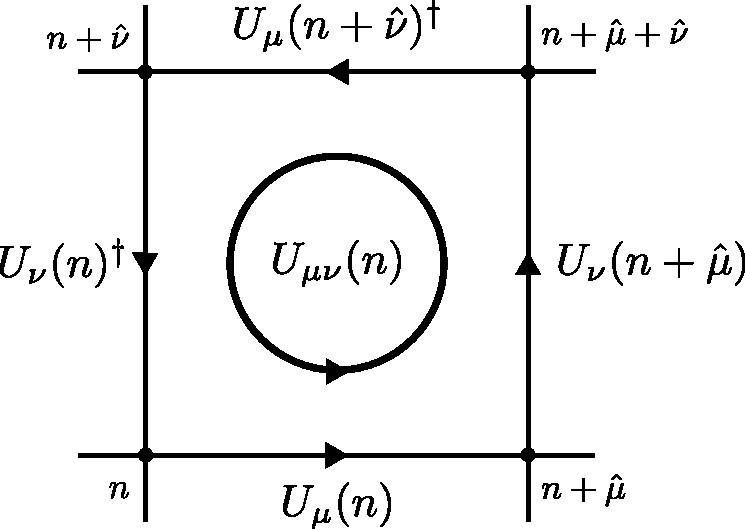
\includegraphics[width=0.5\linewidth]{images/plaquette.pdf}
    \caption{The smallest non-trivial loop on the lattice.}
    \label{fig:plaquette}
\end{figure}
Using this expression we can define a lattice version of the gauge action. To this end we first have to express the plaquette via the continuum variable $A_\mu$ instead of the link variables using equation \eqref{eq:linkVarAndGluonField}. Since the arguments of the exponential functions are matrices we have to use the Baker-Campbell-Hausdorff formula to reduce the product of exponentials to a single exponential. After expanding all gluon fields at the lattice site $n$ to linear order we are left with the approximation
\begin{align}
    U_{\mu\nu}(n)&=\exp\rbr{ia^2(\partial_\mu A_\nu(n)-\partial_\nu A_\mu(n))+i\sqbr{A_\mu(n),A_\nu(n)}+\mathcal O(a^3)}\\
    &=\exp(ia^2G_{\mu\nu}(n)+\mathcal{O}(a^3)).
\end{align}
The lattice gauge is now defined as
\begin{equation}
    S_G[U]=\frac{2}{g^2}\sum_{n\in\Lambda}\sum_{\mu<\nu}\text{Re tr}\sqbr{\mathbb1-U_{\mu\nu}(n)}.
\end{equation}
To see that this expression converges to the continuum action for $a\to0$ we expand the exponential function and use the anti-symmetry of the exponent
\begin{align}
    &\frac{2}{g^2}\sum_{n\in\Lambda}\sum_{\mu<\nu}\text{Re tr}\sqbr{\mathbb1-U_{\mu\nu}(n)}\\
    =&\frac{1}{g^2}\sum_{n\in\Lambda}\sum_{\mu<\nu}\rbr{\text{tr}\sqbr{\mathbb1-U_{\mu\nu}(n)}+\text{tr}\sqbr{\mathbb1-U_{\mu\nu}^\dagger(n)}}\\
    =&\frac{1}{g^2}\sum_{n\in\Lambda}\sum_{\mu<\nu}\rbr{\text{tr}\sqbr{\mathbb1-U_{\mu\nu}(n)}+\text{tr}\sqbr{\mathbb1-U_{\nu\mu}(n)}}\\
    =&\frac{1}{g^2}\sum_{n\in\Lambda}\sum_{\mu,\nu}\text{tr}\sqbr{\mathbb1-U_{\mu\nu}(n)}\\
    =&\frac{1}{g^2}\sum_{n\in\Lambda}\sum_{\mu,\nu}\text{tr}\sqbr{\mathbb1-\mathbb 1 -ia^2G_{\mu\nu}(n)+\frac{a^4}{2}G_{\mu\nu}^2(n)+\mathcal{O}(a^6)}\\
    =&\frac{1}{g^2}\sum_{n\in\Lambda}\sum_{\mu,\nu}\text{tr}\sqbr{-ia^2G_{\mu\nu}(n)}+\text{tr}\sqbr{\frac{a^4}{2}G_{\mu\nu}^2(n)}+\mathcal{O}(a^6)\\
    =&\frac{a^4}{2g^2}\sum_{n\in\Lambda}\sum_{\mu,\nu}\text{tr}\sqbr{G_{\mu\nu}^2(n)}+\mathcal{O}(a^2).
\end{align}
In the limit the sum together with the $a^4$ becomes an integral and the error goes to 0 resulting in the continuum action. Note that $G_{\mu\nu}^2$ is to be understood as squaring the matrix element and we explicitly write the sum over the indices, while in \eqref{eq:qcdLagr} the notation used implicitly summed over the indices\cite{gattringer}.
\todoin{Show that this expression is in the limit the same as the continuum version}

\subsection{Symanzik Improvement: Lüscher-Weisz Gauge Action}
The Wilson Gauge Action goes to the continuum action in the limit. But for finite lattice spacing $a$ the action has an error of order $\mathcal O (a^2)$. The choice of the lattice action is not unique, and there are multiple ways of defining them as long as they converge to the continuum version in the limit. To improve the results of the lattice calculations, it would be favorable to reduce the error. This is the goal of the Symanzik improvement program. The idea is to add more terms and to choose the coefficients in such a way that the leading error is canceled. A typical example is the idea of improving the first order derivative approximation by adding terms that are used to approximate the third derivative. This results in an error that is two orders smaller in $a$.\\
Martin Lüscher and Peter Weisz used this program to improve the Wilson gauge action. Instead of using only all plaquettes on the lattice, they defined the Lüscher-Weisz action by also looking at all (planar) rectangles, parallelograms and bent rectangles, as can be seen in figure \ref{fig:luescherLoops}. In their paper \cite{luscherWeiszAction} they have shown that at tree level we only need to consider the square and rectangular loops to cancel the $\mathcal{O}(a^2)$ error of the Wilson gauge action. The Lüscher-Weisz action is given by
\begin{equation}
    S_{G,LW}=\frac{2}{g^2}\cbr{\frac{5}{3}\sum_\square\text{tr } \sqbr{\mathbb 1-U(\square)}-\frac{1}{12}\sum_\rectangle \text{tr}\sqbr{\mathbb 1-U(\rectangle)}}.
\end{equation}
$U(\square)$ is to be understood as the plaquette defined in equation \eqref{eq:plaquette} and $U(\rectangle)$ is constructed analogously. We sum over all squares but treat squares that differ only in their orientation (e.g. $U_{\mu\nu}$ and $U_{\nu\mu}$) as the same and we do the same for the rectangles.

\begin{figure}
    \centering
    \includegraphics[width=0.5\linewidth]{images/luescherLoops.png}
    \caption{Loops considered in the improved gauge action.}
    \label{fig:luescherLoops}
\end{figure}

\todoin{introduce the idea of tadpole improvement and then introduce the action}

%\subsection{The Haar Measure}
\todoin{still thinking about how much i should mention about it (or if i should mention it at all)}


\section{The Fermionic Part of the Action}
\todoin{Fermions are complicated, and even more on the lattice}

\subsection{Wilson Fermion Action}
Discretizing the fermionic part of the QCD action
\begin{equation}
    S_F =\int d^4x\,\bar\psi(x)\rbr{\slashed D +m}\psi(x) 
\end{equation}
could be done naively by substituting the continuum derivative by the symmetric finite difference quotient and then include link variables to ensure the gauge invariance. This leads to the naive lattice fermion action
\begin{equation}
    S_{\text{F,naive}}=a^4\sum_{n\in\Lambda}\bar\psi(n) \rbr{\gamma_\mu\frac{U_\mu(n)\psi(n+\hat\mu)-U_{-\mu}(n)\psi(n-\hat\mu)}{2a}+m\psi(n)}.
\end{equation}
To see the problem with this formulation we rewrite the expression while stating all indices (except the fermion flavor) explicitly 
\begin{align}
    a^{-4}S_{\text{F,naive}}=\sum_{n,m\in\Lambda}\bar\psi(n)_{a\alpha} D(n|m)_{ab\alpha\beta}\psi(m)_{b\beta}
\end{align}
with
\begin{equation}
    D(n|m)_{ab\alpha\beta}=\rbr{\gamma_\mu}_{\alpha\beta}\frac{U_\mu(n)_{ab}\delta_{n+\hat\mu,m}-U_{-\mu}(n)_{ab}\delta_{n-\hat\mu,m}}{2a}+m\delta_{nm}\delta_{ab}\delta_{\alpha\beta}.
\end{equation}
Following the derivation in \cite{gattringer} we can compute the Fourier transform of $D(n|m)$ for the case of setting all link variables to unity
\begin{align}
    \tilde{D}(p|q)&=\frac{1}{\lvert\Lambda\rvert}\sum_{n,m\in\Lambda}e^{-ipna}D(n|m)e^{iqma}\\
    &=\delta(p-q)\rbr{m\mathbb 1 +\frac{i}{a}\sum_\mu\gamma_\mu\sin(p_\mu a)}\\
    &=\delta(p-q)\tilde D(p).
\end{align}
For $m=0$ the inverse is given by
\begin{equation}
    \tilde D(p)^{-1}=-ia\frac{\sum_\mu\gamma_\mu\sin(p_\mu a)}{\sum_\mu\sin(p_\mu a)^2}.
\end{equation}
This is the propagator whose poles describe particles. In the continuum limit $a\to0$ the only pole is for $p=0$. For non-zero $a$ however, we get a pole when $\sin(p_\nu a)$ is zero for all $\nu$. On the lattice the momentum range in every direction is $(-\pi/2,\pi/2]$, giving rise to 16 poles. These lattice artifacts are called fermion doublers, since we have 16 fermions for every single physical fermion\cite{gattringer}. 

\todoin{write the naive version by substituting the continuum derivative by its lattice counterpart.}
\todoin{Link variables and their transformation}
\todoin{maybe the connection the link variables and the field via gauge transporter}

\subsection{Wilson Fermion Action}
To remove these doublers Wilson introduced an additive term, the Wilson term, so that the Fourier transform becomes
\begin{equation}
    \tilde D(p)=m\mathbb1+\frac{i}{a}\sum_\mu\gamma_\mu\sin(p_\mu a)+\mathbb1\frac{1}{a}\sum_\mu\rbr{1-\cos(p_\mu a)}.
\end{equation}
This extra term vanishes for $p=0$ while it adds the term $\frac2a$ for each momentum component taking the value $\frac{\pi}{a}$ which can be thought of as an additional mass term. In the continuum limit this new mass diverges and these extra poles decouple from the theory leaving us with a single fermion\cite{gattringer}.

\todoin{Fermion doubling problem and its solution with the extra term}
\subsection{Chiral symmetry and the Nielsen-Ninomiya theorem}
The QCD Lagrangian satisfies the chiral symmetry in the massless case, which is also the reason why we call this case the chiral limit. In the continuum this symmetry implies that the Lagrangian does not change when we rotate the spinor fields according to
\begin{equation}
    \psi^\prime=\exp(i\alpha\gamma_5)\psi,\qquad \bar\psi^\prime=\bar\psi\exp(i\alpha\gamma_5)
\end{equation}
introducing the fifth gamma matrix
\begin{equation}
    \gamma_5:=\gamma_1\gamma_2\gamma_3\gamma_4
\end{equation}
which anticommutes with the other gamma matrices
\begin{equation}
    \cbr{\gamma_5,\gamma_\nu }=0.
\end{equation}
Using this property, it follows that in the chiral limit the symmetry is fulfilled. This symmetry and its spontaneous breaking explain important mass related properties in QCD and cannot be simply ignored.\\
On the lattice we loose the chiral symmetry in Wilson's formulation even in the massless case. The reason for this is that the Wilson term behaves like a mass term and thus breaks the symmetry exactly like the mass term outside the chiral limit.\\
The Nilesen-Ninomiya theorem destroys the hope that by choosing another way of discretizing the theory, we may overcome this problem. It states that on the lattice we cannot ensure chiral symmetry and remove the fermion doublers at the same time. \\
One way of solving this problem is to define a lattice version of the chiral symmetry that goes into the continuum version for $a\to 0$. Another approach that has other problems but is computationally faster is the staggered fermion formulation\cite{gattringer}.


\subsection{(Highly Improved) Staggered Quark action}
\todoin{I am still thinking about this}

In the staggered fermions formulation, which are also called Kogut-Susskind fermions, we keep the continuum chiral symmetry while reducing the number of fermion doublers from 16 to four. The idea is to transform the spinor field so that the Dirac operator is diagonal in spinor space so that we can discard all but one component. \\
We start by performing a position dependent rotation of the Dirac spinors in the spinor space
\begin{equation}
    \psi(n)=\gamma_1^{n_1}\gamma_2^{n_2}\gamma_3^{n_3}\gamma_4^{n_4}\psi(n)',\quad \bar\psi(n)=\bar\psi(n)'\gamma_4^{n_4}\gamma_3^{n_3}\gamma_2^{n_2}\gamma_1^{n_1}
\end{equation}
with
\begin{equation}
    n=(n_1,n_2,n_3,n_4).
\end{equation}
Since the square of each gamma matrix is just the identity, it follows that the mass term is invariant under this rotation. The derivative term transforms non-trivially since it contains gamma matrices and compares fields at different lattice sites. Using the Clifford algebra we find
\begin{align}
    \bar\psi(n)\gamma_1\psi(n\pm\hat1)&=\bar\psi(n)'\mathbb1\psi(n\pm\hat1)'\\
    \bar\psi(n)\gamma_2\psi(n\pm\hat2)&=\bar\psi(n)'\mathbb1\psi(n\pm\hat2)'(-1)^{n_1}\\
    \bar\psi(n)\gamma_3\psi(n\pm\hat3)&=\bar\psi(n)'\mathbb1\psi(n\pm\hat3)'(-1)^{n_1+n_2}\\
    \bar\psi(n)\gamma_4\psi(n\pm\hat4)&=\bar\psi(n)'\mathbb1\psi(n\pm\hat4)'(-1)^{n_1+n_2+n_3}
\end{align}
with $\hat i$ denoting one step in the $i$ direction. Introducing the staggered sign function $\eta_\mu(n)$ we may summarize the previous equations via
\begin{equation}
    \bar\psi(n)\gamma_\mu\psi(n\pm\hat\mu)=\eta_\mu(n)\bar\psi(n)\psi(n\pm\hat\mu).
\end{equation}
The naive fermion Lagrangian expressed in the transformed fields reads
\begin{equation}
    \lagr(\psi, \bar\psi)=\bar\psi(n)'\mathbb1\rbr{\sum_\mu\eta_\mu(n)\frac{\psi(n+\hat\mu)'-\psi(n-\hat\mu)'}{2a}+m\psi(n)'}.
\end{equation}
The Dirac operator is now diagonal in the spinor space. Thus, we may keep only one component and receive the staggered fermion action 
\begin{equation}
    S_F[\chi,\bar\chi]=a^4\sum_{n\in\Lambda}\bar\chi(n)\rbr{\sum_\mu\frac{U_\mu(n)\chi(n+\hat\mu)-U_{-\mu}(n)\chi(n-\hat\mu)}{2a}+m\chi(n)}.
\end{equation}
To see that the action satisfies the chiral symmetry (in the chiral limit), we first need to find the corresponding chiral transformation for the transformed fields. Using once again the commutation relations of the gamma matrices, we find
\begin{equation}
    \bar\psi(n)\gamma_5\psi(n)=(-1)^{n_1+n_2+n_3+n_4}\bar\psi(n)'\psi(n)'=:\eta_5(n)\bar\psi(n)'\psi(n)'.
\end{equation}
In the chiral limit this means that our new fields transform via
\begin{equation}
    \chi(n)'=\exp(i\alpha\eta_5(n))\chi(n),\quad\bar\chi(n)'=\exp(i\alpha\eta_5(n))\bar\chi(n)
\end{equation}
and the chiral symmetry follows as can be seen from
\begin{align}
    &\bar\chi(n)'\chi(n\pm\hat\mu)'\\
    =&\bar\chi(n)'e^{i\alpha\eta_5(n)}e^{i\alpha\eta_5(n\pm\hat\mu)}\chi(n\pm\hat\mu)'\\
    =&\bar\chi(n)\chi(n\pm\hat\mu)\exp\sqbr{i\alpha\rbr{(-1)^{n_1+n_2+n_3+n_4}+(-1)^{n_1+n_2+n_3+n_4\pm1}}}\\
    =&\bar\chi(n)\chi(n\pm\hat\mu).
\end{align}
Since the staggered fermions are Grassmann variables we may use the same trick to write the integral over the fermions fields as the fermion determinant. Since we still have four fermions for each physical fermion, which are called tastes, it is common practice to take the fourth root of the determinant.\\
In our simulations we will not use the staggered fermion action, but the Highly Improved Staggered Quark (HISQ) action\cite{hisq}. This improved action eliminates tree level errors resulting from taste exchange interactions by smearing the link variables and finite difference errors of order $\mathcal O(a^2)$ by including further terms.\cite{bielefeldPHD}\newpage

\chapter{Statistical Physics and Thermodynamics}The partition function was already introduced in section \ref{sec:pathIntPartFunc} as the trace over the density matrix
\begin{equation}
    Z=\tr\hat\rho=\tr\exp(-\beta_T\hat{H}),
\end{equation}
and we have seen after the Wick rotation we can write the function via a path integral. An important detail is that $\beta_T$ sets the upper bound of the temporal integration, which means that we introduce temperature into the system by limiting the integration range. If we would integrate up to infinity the temperature $T=1/\beta_T$ goes to zero corresponding to the vacuum. Since we have to send the volume to infinity to get physical results we cannot have the same number of lattice points in space and temporal direction. We write
\begin{equation}
    T=\frac{1}{N_Ta},\quad V=(N_Sa)^3,\quad \frac{V}{T}=a^4N_TN_S^3
\end{equation}
with the $N_T$ the number of lattice sites in temporal direction and $N_S$ the number of points in each space direction and $a$ the usual lattice spacing.\\
In the following discussion we will use the simplified partition function
\begin{equation}
    Z(\beta,m)=\int \mathcal DU \det[\slashed D+m]\exp\rbr{-\beta S_G[U]}\label{eq:simpleZ}
\end{equation}
with $\beta=6/g^2$ the lattice gauge coupling.
\section{The Partition Function and Bulk Quantities}

This object entails all statistical information of the system. It can be used to calculate bulk quantities such as the pressure, the entropy and the energy\cite{kapusta}
\begin{equation}
    P=\frac{\partial T\ln Z}{\partial V},\quad S=\frac{\partial(T\ln Z)}{\partial T},\quad E=-PV+TS.   
\end{equation}
In the thermodynamical limit the expression for the pressure simplifies to 
\begin{equation}
    p=\frac{T}{V}\ln Z.
\end{equation}
A useful quantity is the trace anomaly
\begin{equation}
    I=3P-\epsilon=-T^5\frac{\partial}{\partial T}\frac{P(T)}{T^4},
\end{equation}
because it can be computed from the pressure alone and can be used to calculate the energy density $\epsilon$ afterwards. Using these quantities we can also compute the entropy density $s$ and the speed of sound $c_s$
\begin{equation}
    s=\frac{P+\epsilon}{T},\quad c_s^2=\frac{dP}{d\epsilon}.
\end{equation}
This means that if we could calculate the partition and take its derivative we can extract the pressure and then all other bulk quantities. The problem is that in lattice QCD we cannot calculate $Z$ directly but only expectation values. However, derivatives of $\ln Z$ are nothing but expectation values. Thus, by integrating over the derivatives of $\ln Z$ we can reconstruct the partition function and thus the pressure\cite{integralMethod}.


\section{Integral Method}
The Integral Method\cite{firstIntegralMethod} was proposed as a non-perturbative way to analyze thermodynamic quantities such as pressure without having to rely on perturbative calculations of the gauge coupling. \\
Since measurements on the lattice must be dimensionless, we introduce the dimensionless pressure
\begin{equation}
    P^{\text{lat}}=Pa^4=\frac{1}{N_TN_S^3}\ln Z.
\end{equation}
We introduce a parameter $\lambda$ for $\beta(\lambda)$ and $m(\lambda)$ so that the pressure and partition function depend only on $\lambda$. Invoking the fundamental theorem of calculus and using the chain rule we have
\begin{align}
    P^{\text{lat}}(\beta, m)-P^{\text{lat}}(\beta_0,m_0)&=\frac1{N_TN_S^3}\int_{\lambda_0}^{\lambda}d\lambda'\frac{\partial \ln Z}{\partial \lambda'}\\
    &=\frac{1}{N_TN_S^3}\int_{(\beta_0,m_0)}^{(\beta,m)}\rbr{d\beta'\frac{\partial\ln Z}{\partial \beta'}+dm'\frac{\partial \ln Z}{\partial m'}}.
\end{align}
The derivative of the logarithm of equation \eqref{eq:simpleZ} leads to
\begin{align}
    \frac{\partial \ln Z}{\partial \beta}&=\frac{1}{Z}\int \mathcal DU \det[\slashed D+m]\exp\rbr{-\beta S_G[U]} (-S_G[U])\\
    &=\langle-S_G\rangle.
\end{align}
For the second term we need to use Jacobi's formula
\begin{equation}
    \frac{d\det A(\lambda)}{d\lambda}=\det A(\lambda)\cdot\tr\rbr{A^{-1}\frac{dA}{d\lambda}}
\end{equation}
to get
\begin{align}
     \frac{\partial \ln Z}{\partial m}&=\frac{1}{Z}\int \mathcal DU \det[\slashed D+m]\exp\rbr{-\beta S_G[U]} \tr\frac{1}{\slashed D+m}\\
     &=\left\langle\tr\frac{1}{\slashed D+m}\right\rangle.
\end{align}
When would calculate the derivative with respect to the mass of the expression in which the Grassmann integration was not yet done, only the mass term of the fermionic action depends on the mass and we get alternatively
\begin{equation}
     \frac{\partial \ln Z}{\partial m}=\langle\bar\psi\psi\rangle
\end{equation}
which is called the chiral condensate. Putting all together we have
\begin{equation}
    P^{\text{lat}}(\beta, m)-P^{\text{lat}}(\beta_0,m_0)=\frac{1}{N_TN_S^3}\int_{(\beta_0,m_0)}^{(\beta,m)}\rbr{d\beta'\langle-S_G\rangle+dm'\langle\bar\psi\psi\rangle}. 
\end{equation}
We finish this section with a few notes. Firstly, one may take the factor of the integral inside the expectation value to have expectation values of densities. Secondly, it is important that the same calculation is done again with a much lower temperature to cancel additive divergences that would appear otherwise. We will do this by repeating the calculation for half the temperature. Thirdly, while this method allows the calculation of the pressure for given gauge coupling and mass, we still need to have the pressure for some other parameter combination. We will solve this problem by choosing our starting point at $m=\infty$ and $\beta=\infty$ where we know the pressure. Lastly, the parameter dependence of $\beta$ and $m$ are often chosen in a way that the parameter path goes along a Line of Constant Physics. This means along these path all calculations give rise to valid physical results. But this path has the problem that the calculations are more expensive and give rise to bigger errors than the path that we choose. But since only the end point matters, our path, which uses unphysical intermediate steps such as quarks with infinite masses, is a valid path. \cite{integralMethod}

\todoin{Start with saying that we cannot calculate Z, only expectation values (and derivatives)}
\todoin{Using Derivatives requires to integrate from a known point to the point of interest.}
\todoin{Talk about possible paths that we might take}

%\subsection{Non-Thermal}
\todoin{Instead of calculating derivatives via expectation values we can calculate expectation values themselves along a path without thermalization}
\todoin{We talked about two ways, and i am unsure if I should include Jarzynskis way since it seemed to be the worse one}\newpage

\chapter{The Measuring Process}                 When we want to calculate the expectation values of some quantity $O$ in the pure gauge theory we need
\begin{equation}
    \langle O\rangle=\frac{1}{Z} \int\mathcal D[U]\exp\rbr{-S_G[U]}O[U],\quad Z=\int \mathcal D[U]\exp\rbr{-S_G[U]}.
\end{equation}
Instead of evaluating this infinite dimensional integral analytically we may approximate it by a Monte-Carlo integration. We choose $N$ configurations $U_n$ according to the probability density 
\begin{equation}
    dF[U]=\frac{\exp(-S_G[U])\mathcal D[U]}{\int\mathcal D[U']\exp(-S_G[U'])}
\end{equation}
and evaluate
\begin{equation}
    \frac{1}{N}\sum_{n=1}^NO[U_n].
\end{equation}
The statistical error is proportional to $1/\sqrt{N}$ and in the limit $N\to\infty$ we have
\begin{equation}
    \langle O\rangle=\underset{N\to\infty}{\lim}\frac{1}{N}\sum_{n=1}^NO[U_n]
\end{equation}
\cite{gattringer}.
\section{Markov chains and the Metropolis algorithm}

To approximate the expectation value we need to generate many configurations. We generate these via a Makrov process. This means that we generate configurations subsequently, with each following configuration depending only on the previous one, ignoring the previous history. This is schematically shown in figure \ref{fig:markov}. The probability of choosing a new configuration is called transition probability $T(U|U')$. We start with an arbitrary configuration $U_0$ which means that our configuration distribution is simply $P^{(0)}(U)=\delta(U-U_0)$. Each time we generate a new configuration we let $T$ act on the distribution resulting in a new configuration. This is the thermalization process in which the configuration distribution differs from the actual physical distribution. Using these configurations to compute the expectation value would lead to wrong values. Instead we will keep generating new configurations until thermalization is over and the configuration distribution is in equilibrium. This is the case if in the step $n\to n+1$ the probability of $U'$ being the new configuration is the same as the probability of $U'$ being the old configuration. This condition is the balance equation
\begin{equation}
    \sum_UT(U'|U)P(U)\overset{!}{=}\sum_UT(U|U')P(U').
\end{equation}
Using the normalization of the transition probability
\begin{equation}
    \sum_UT(U|U')=1
\end{equation}
the balance equation becomes
\begin{equation}
    \sum_UT(U'|U)P(U)=P(U')
\end{equation}
which means that our equilibrium distribution is a fixed point of $T$. It is necessary to ensure that $T(U|U')$ is strictly positive to make every configuration reachable from every starting point and make the Markov chain aperiodic. This strong ergodicity guarantees that our configuration distribution converges to the equilibrium distribution, as long as the transition probability satisfies the balance equation. One way of enforcing this is by expecting the transition probability $T$ to satisfy the condition for each term. This sufficient condition is called detailed balance 
\begin{equation}
    T(U'|U)P(U)=T(U|U')P(U')
\end{equation}
and this will be used here.\\
\begin{figure}[H]
    \centering
    \includegraphics[width=0.7\linewidth]{images/markov.png}
    \caption{Example of a Markov chain. In every step a new configuration is chosen. ll possible configurations are inside the boundary\cite{gattringer}.}
    \label{fig:markov}
\end{figure}
The generation of configurations is now done following the Metropolis algorithm consisting of the repetition of two steps
\begin{enumerate}
    \item Choose a candidate configuration $U'$ according to an a priori selection probability $T_0(U'|U)$
    \item Accept $U'$ with a probability $T_A(U'|U)=\min\rbr{1,\frac{T_0(U|U')\exp(-S[U'])}{T_0(U'|U)\exp(-S[U])}}$.
\end{enumerate}
The combined probability $T=T_0T_A$ satisfies the detailed balance condition using $P(U)\propto\exp(-S[U])$. When we choose a symmetric selection probability $T(U|U')=T(U'|U)$, the accept probability reduces to
\begin{equation}
    T_A=\min(1,\exp(-\Delta S)),\quad\Delta S=S[U']-S[U],\label{eq:acceptProb}
\end{equation}
meaning it depends only on the difference in action. \\
The generation of a configuration candidate can be expensive and often it is rejected. But we can use that the acceptance probability depends only on the change in action to improve the computation time. In the pure gauge case for example we may take the same configuration and change only one link variable $U_\mu(n)'$. The difference in action depends only on the change in 6 plaquettes which include this link variable 
\begin{equation}
    S_{loc}=\frac{\beta}{3}\sum_{i=1}^6\text{Re }\tr\sqbr{\mathbb1-U_\mu(n)'P_i}=\frac{\beta}{3}\text{Re }\tr\sqbr{6\mathbb1-U_\mu(n)'A}.
\end{equation}
The $P_i$ denote the 6 plaquettes excluding the new link variable, which are called staples, and $A$ is given 
by their sum
\begin{align}
    A=\sum_{i=1}^6P_i=\sum_{\nu\neq\mu}\big(&U_\nu(n+\hat\mu)U_{-\mu}(n+\hat\mu+\hat\nu)U_{-\nu}(n+\hat\nu)\\
    +&U_{-\nu}(n+\hat\mu)U_{-\mu}(n+\hat\mu-\hat\nu)U_{\nu}(n-\hat\nu)\big).
\end{align}
The staples are the same in the proposed configuration and the action difference is
\begin{equation}
    \Delta S=-\frac{\beta}{3}\text{Re }\tr\sqbr{\rbr{U_\mu(n)'-U_\mu(n)}A}.
\end{equation}
If we now have a configuration candidate, in this one link variable, we may now accept or reject it with the probability \eqref{eq:acceptProb}\cite{gattringer}. \\
%Now we look at how we generate the candidates, but for this we need to understand how to represent link variables. While our link variables are elements of $SU(3)$, we will not use algorithms that generate these matrices, but matrices in $SU(2)$ and use them to build $SU(3)$. 


\todoin{Markov chains and general metropolis}
\todoin{generating random numbers}

\section{Simulation in Pure Glue: Heat Bath and Overrelaxation}
We will use two algorithms to generate link variable configurations: the heat bath algorithm and overrelaxation. In principle, the first algorithm is enough, but like in the previous section we change the link variables only one by one. Thus, it takes a long time to get uncorrelated configurations which are needed for the computation of expectation values. Overrelaxiation leads to big changes, however, it keeps the action unchanged, which means that this algorithm alone does not satisfy ergodicity which is needed to explore the full configuration space. It is therefore common practice to use a combination of both algorithms to use both advantages.\\
While these algorithms are used to generate our link variables which are elements of $SU(3)$, they actually produce multiple $SU(2)$ matrices which are used to generate the $SU(3)$ matrix. The reason for this is that the algorithms use the fact that the sum of $SU(2)$ matrices are proportional to another $SU(2)$ matrix. This property is not true for the higher dimensional case.\\
While the Metropolis algorithm starts by the generation of a candidate configuration according to some selection probability and then accepts it with a acceptance probability, the heat bath algorithm directly generates link variables that are distributed correctly according to
\begin{equation}
    dP(U)=dU\exp\rbr{\frac{\beta}{N}\text{Re} \tr\sqbr{UA}}.
\end{equation}
Using the invariance of the measure $dU$ under transformation and the aforementioned property that we may write the sum of $SU(2)$ matrices as
\begin{equation}
    A=:\sqrt{\det\sqbr{A}}V=:aV
\end{equation}
with $V\in SU(2)$, we can rewrite the distribution
\begin{equation}
    dP(X)=dX\exp\rbr{\frac{a\beta}{2}\text{Re }\tr\sqbr{X}}
\end{equation}
and then calculate
\begin{equation}
    U=XV^\dagger=XA^\dagger\frac{1}{a}.
\end{equation}
Since this is for the computation for $SU(2)$ matrices we have used $N=2$.\\
We will not show how to generate $X$ according to this distribution since it requires talking about the Haar measure $dU$ and other technical details regarding the extraction of random numbers from different distributions. Instead we refer to \cite{gattringer}. The literature also explains how we can construct the $SU(3)$ link variable by using the algorithm thrice.\\
Overrelaxation also skips the accept/reject step by choosing configurations that do not change the action, which implies that the acceptance date is 100 percent. In $SU(2)$ this can be done by changing the link variables according to
\begin{equation}
    U'=V^\dagger U^\dagger V^\dagger
\end{equation}
with $V$ being again the normalization of the staples $A$. Using that $SU(2)$ matrices have real traces and their unitarity we have
\begin{equation}
    \tr\sqbr{U'\cdot A}=\tr\sqbr{V^\dagger U^\dagger V^\dagger\cdot Va}=\tr\sqbr{A^\dagger U^\dagger}=\tr\sqbr{UA}.
\end{equation}
Since the trace does not change, the action does not change as well and this new configuration is accepted.\\
Using both algorithms we can then change the configuration significantly using overrealaxation, while needing heat bath to explore regions of the configuration space that have other actions and are therefore not reachable with overrelaxation alone\cite{gattringer}. 
\section{Simulation in Full QCD: Hybrid Monte Carlo}
\subsection{Fermion determinant and pseudofermions}
Up until now we have only considered the generation of the gluonic part of the configurations. When we include (dynamic) fermions we have to include the fermion determinant in our calculations. The idea of treating the determinant as part of the observable and ignoring it during the process of generating the configurations fails because the determinant fluctuates over several orders of magnitude. Instead it has to be used as a weight factor of the distribution. This can give rise to problems, since the fermion determinant is generally not positive, which leads to the sign-problem. Since we do not include the chemical potential in our calculations and our Dirac operator has sufficient properties such as chirality and $\gamma_5$-hermiticity, we are ensured that the determinant is positive.\\
The fermion determinant was the result of a Grassmann integration of a Gaussian. Assuming two mass-degenerate quark flavors we have
\begin{align}
    &\int\mathcal D\psi^{(u)}\mathcal D\bar\psi^{(u)}\mathcal D\psi^{(d)}\mathcal D\bar\psi^{(d)} \exp(-\bar\psi^{(u)}D\psi^{(u)}-\bar\psi^{(d)}D\psi^{(d)}\\ =&\det\sqbr{D}\det\sqbr{D}=\det\sqbr{D}\det\sqbr{D^\dagger}=\det\sqbr{DD^\dagger}.
\end{align}
But we can also write 
\begin{equation}
    \det\sqbr{DD^\dagger}=\pi^{-N}\int\mathcal D\phi_I\mathcal{D}\phi_R\exp\rbr{-\phi^\dagger\rbr{DD^\dagger}^{-1}\phi}
\end{equation}
for complex field with $N$ components 
\begin{equation}
    \phi=\phi_R+i\phi_I. 
\end{equation}
These are normal complex fields, meaning they behave like bosons. Since we can use them to describe fermions we call them pseudofermions. The action is now given by
\begin{equation}
    S[U,\phi]=S_G[U]+\phi^\dagger(DD^\dagger)^{-1}\phi.
\end{equation}
The reason for using the determinant for mass-degenerated quarks is that the following algorithm needs the positivity of $DD^\dagger$ but $D$ is not positive.  
\subsection{Hybrid Monte Carlo}
The heat bath algorithm, which can be used in the pure glue case, used the fact, that when we change a single link variable this only effects its neighborhood. This local property is not true once we include the fermion determinant. Since this implies that the computation is expensive, we could simply change a lot of link variables at once. But this has the downside of leading to low acceptance rates. Instead we will use the idea of overrelaxation of enforcing a high acceptance rate by (almost) not changing the action via the new configuration. This is done by imitating the dynamics of classical particles with coordinates and conjugate momenta who evolve in a way that do not change the Hamiltonian and in our case the action. The coordinates $Q$ are related to the link variables $U$ while the momenta $P$ are introduced by multiplying by a one. The dynamics of the Hamiltonian 
\begin{equation}
    H[Q,P]=\frac{1}{2}P^2+S[Q]
\end{equation}
are governed by the equations
\begin{equation}
    \dot P =-\frac{\partial H}{\partial Q},\qquad \dot Q=P,
\end{equation}
which can be solved numerically, with the initial values of $P$ being drawn from a Gaussian distribution. While we can extract from these $Q$ the new configuration, we remind ourselves that we need to ensure the detailed balance equation if we want the Markov process to thermalize. It can be shown that solving the differential equations via the leapfrog algorithm satisfies the condition.\\
Leaving aside the technical details of the implementation, the hybrid Monte Carlo algorithm starts with drawing the pseudofermion fields from a Gaussian distribution. Then the conjugate momenta are also drawn from a Gaussian distribution and used to solve the Hamilton equations to compute new link variable candidates. Since we solve the differential equations numerically we introduce errors which lead to a change in the action. Thus, we only accept the configuration according to the acceptance probability.\\
The above sketch follows \cite{gattringer} but ignores two points that are important for this thesis. Firstly, the algorithm assumes an even number of mass-degenerate quark flavors, however, while we assume that the up and down quark have the same mass, we also take into account the strange quark, which has a much higher mass. So we have an odd number of quarks and they are not mass-degenerate. Secondly, we do not use quark spinors but staggered fermions. This requires that we have to take the fourth root of the strange determinant and the second root of the light quark determinant. Therefore, we will not use the standard HMC algorithm but the rational hybrid Monte Carlo algorithm, where the root of the determinant is approximated by a rational function\cite{bielefeldPHD}.

\newpage

\chapter{Set Up and Outlook}                In this final section we will shortly sum up our set up and mention how we want to measure the pressure.\\
We are following the set up in \cite{eos2_1}. We choose for our lattice action the HISQ/tree action for $N_f=2+1$ fermions. This means that we choose for the gauge action the Lüscher-Weisz action, also known as the tree level symanzik improved gauge action, which gives rise to the parameters $\beta_\square$ and $\beta_\rectangle$. The fermion action is the highly improved staggered quark action. We assume that the up and down quark have the same mass $m_l$ and we have as a second parameter the strange quark mass $m_s$.\\
The pressure is measured using the integral method along paths that are described below. The integral method requires the calculation of expectation values which will be done using Rational Hybrid Monte Carlo integration when including dynamical (staggered) fermions.\\
We want to calculate the pressure at roughly 400 MeV. At this scale we are above the critical temperature which is at roughly 155 MeV where the phase transition between confinement and deconfinement occurs. Furthermore, when we do the measurement at half the temperature to subtract the divergences we are still above the critical temperature. To do the continuum limit we choose the following three parameter combinations to respect the line of constant physics.
\begin{table}[h]
\centering
\begin{tabular}{c c c c c c}
\hline
$\beta$ & $m_l$ & $m_s$ & $n_\tau$ & $T$ (MeV) \\
\hline
7.373 & 0.00125 & 0.0250 & 8  & 409.7 \\
7.596 & 0.00101 & 0.0202 & 10 & 400.0 \\
7.825 & 0.00082 & 0.0164 & 12 & 407.4 \\
\hline
\end{tabular}
\caption{Simulation Parameters and corresponding temperature. We choose $m_l=m_s/20$.}
\label{tab:lattice_params}
\end{table}

For each parameter combination we choose the same paths. In a first step we have to make sure that we do not cross any phase transitions since this would lead to big statistical uncertainties making the measurement useless. If we know that the following paths would not result in crossing the phase transitions, we can continue as planned. Otherwise we have to change the paths in a way to go around the phase transition.\\
\begin{figure}[H]
    \centering
    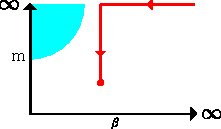
\includegraphics[width=0.7\linewidth]{images/path.pdf}
    \caption{Simplified path going to infinite quark mass and then to infinite lattice gauge coupling. The blue arc marks the area where we would pass a phase transition.}
    \label{fig:path}
\end{figure}
Then we want to go to infinite quark masses so that they decouple from the theory and we can continue in pure glue. Instead of increasing all quark masses in the same way, we will try to first have $SU(3)$ flavor symmetry so that all quarks have the same mass, hoping that this improves the results.\\
Lastly, once we reach pure glue we can either keep using the Lüscher-Weisz action sending both gauge couplings to infinity or we follow a path that switches to the Wilson gauge action which is already well understood. A simplified path can be seen in figure \ref{fig:path}\\
While this is the plan for the measurement of the pressure, we might investigate non-equilibrium integral methods as well if time permits.  
\todoin{Writing down the full expressions and listing the paremters (from pavan)}
\todoin{a plan of all paths we will take and what methods (which integration method and update algorithm)}

\newpage




\bibliography{references}   \bibliographystyle{ieeetr} \newpage

%\appendix \chapter{Appendix}\todoin{lets see if i will need this at all}\newpage

\textbf{Erklärung zur Abschlussarbeit gemäß § 22 Abs. 7 APB TU Darmstadt}

Hiermit erkläre ich, \underline{\textit{Abdelhamid Ettahri}}, dass ich die vorliegende Arbeit gemäß § 22 Abs. 7 APB TU Darmstadt selbstständig, ohne Hilfe Dritter und nur mit den angegebenen Quellen und Hilfsmitteln angefertigt habe. Ich habe mit Ausnahme der zitierten Literatur und anderer in der Arbeit genannter Quellen keine fremden Hilfsmittel benutzt. Die von mir bei der Anfertigung dieser wissenschaftlichen Arbeit wörtlich oder inhaltlich benutzte Literatur und alle anderen Quellen habe ich im Text deutlich gekennzeichnet und gesondert aufgeführt. Dies gilt auch für Quellen oder Hilfsmittel aus dem Internet.

Diese Arbeit hat in gleicher oder ähnlicher Form noch keiner Prüfungsbehörde vorgelegen.

Mir ist bekannt, dass im Falle eines Plagiats (§38 Abs.2 APB) ein Täuschungsversuch vorliegt, der dazu führt, dass die Arbeit mit 5,0 bewertet und damit ein Prüfungsversuch verbraucht wird. Abschlussarbeiten dürfen nur einmal wiederholt werden.\\
\textcolor{black!20}{\makebox[\linewidth]{\rule{\textwidth}{0.4pt}}}\\
\textbf{English translation for information purposes only:\\
\\
Thesis Statement pursuant to § 22 paragraph 7 of APB TU Darmstadt}

I herewith formally declare that I, \underline{\textit{Abdelhamid Ettahri}}, have written the submitted thesis independently pursuant to § 22 paragraph 7 of APB TU Darmstadt without any outside support and using only the quoted literature and other sources. I did not use any outside support except for the quoted literature and other sources mentioned in the paper. I have clearly marked and separately listed in the text the literature used literally or in terms of content and all other sources I used for the preparation of this academic work. This also applies to sources or aids from the Internet.

This thesis has not been handed in or published before in the same or similar form.

I am aware, that in case of an attempt at deception based on plagiarism (§38 Abs. 2 APB), the thesis would be graded with 5,0 and counted as one failed examination attempt. The thesis may only be repeated once.\\
\textcolor{black!20}{\makebox[\linewidth]{\rule{\textwidth}{0.4pt}}}\\

Datum / Date: \hspace{4cm} Unterschrift/Signature:\\                    
\underline{{~~\huge11.03.2026}\phantom{Dat}} \hspace{2cm } 
\underline{\includegraphics[height=40pt]{signature.png}}

\end{document}
